\documentclass[a4paper, 12pt]{report}
\usepackage[utf8]{inputenc}
\usepackage{hyperref}
\usepackage{graphicx}
\usepackage{float}
\usepackage{xcolor}
\usepackage{listings}
\hypersetup{
    colorlinks,
    linkcolor={black!50!black},
    citecolor={blue!50!black},
    urlcolor={blue!80!black}
}

\definecolor{dkgreen}{rgb}{0,.6,0}
\definecolor{dkblue}{rgb}{0,0,.6}
\definecolor{dkyellow}{cmyk}{0,0,.8,.3}

\lstset{
  language        = php,
  basicstyle      = \small\ttfamily,
  keywordstyle    = \color{dkblue},
  stringstyle     = \color{red},
  identifierstyle = \color{dkgreen},
  commentstyle    = \color{gray},
  emph            =[1]{php},
  emphstyle       =[1]\color{black},
  showstringspaces=false
  showspaces=true,
  }
  
\title{Analisi Progetto "Tracking Spedizione"}
\author{Simone Pozzebon - pozze.simo@gmail.com \\"I.T.S.T J.F.Kennedy" \\ Pordenone }
\date{April 2021}

\begin{document}

\maketitle
\newpage
\tableofcontents
\newpage

\section{Testo del problema}
\begin{figure}[H]
    \centering
    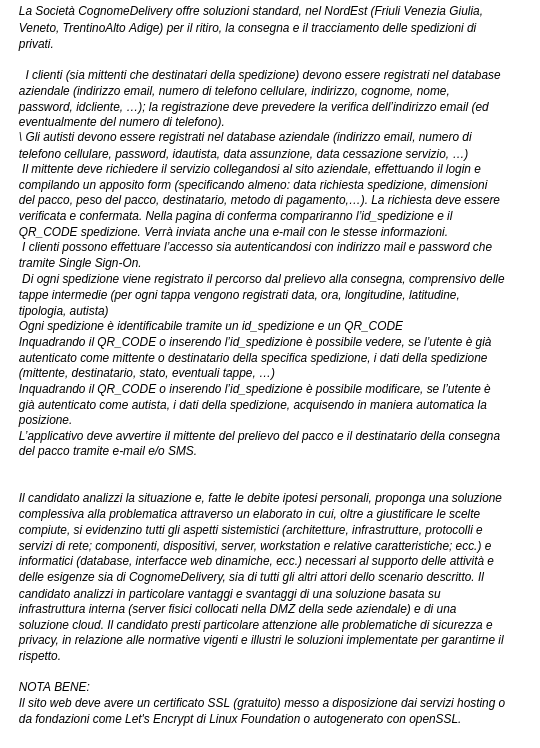
\includegraphics[scale=0.5]{img/testo1.png}
    \caption{Testo}
    \label{fig:my_label}
\end{figure}
\begin{figure}[H]
    \centering
    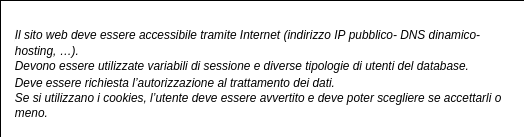
\includegraphics[scale=0.5]{img/testo2.png}
    \caption{Testo}
    \label{fig:my_label}
\end{figure}
\newpage
\section{Soluzione}
\subsection{Introduzione Generale e Funzionalita'}\
La richiesta di tracking dei pacchi per la zona del Nord Est italia e’ stata presa in carico dalla ditta Pozzebon Spa attraverso un portale web. 

Il sito e’ stato interamente ideato, sviluppato e pubblicato da Simone Pozzebon.

Le tecnologie utilizzate sono svariate: Php e JS per gestire il backend del sito in combinazione con Html5 e Css per la gestione dell’interfaccia dell’utente. 

La parte di database e’ stata affidata a mySql, per elaborare le richieste del sito ci si e’ affidati al web-server Apache.
Tutto il portale e’ hostato su piattaforma \href{https://aws.amazon.com/free/?trk=ps_a134p000003yhhNAAQ&trkCampaign=acq_paid_search_brand&sc_channel=ps&sc_campaign=acquisition_IT&sc_publisher=google&sc_category=core&sc_country=IT&sc_geo=EMEA&sc_outcome=Acquisition&sc_detail=amazon%20aws&sc_content=Amazon%20AWS_e&sc_matchtype=e&sc_segment=455721528683&sc_medium=ACQ-P|PS-GO|Brand|Desktop|SU|AWS|Core|IT|EN|Text&s_kwcid=AL!4422!3!455721528683!e!!g!!amazon%20aws&ef_id=CjwKCAjwvMqDBhB8EiwA2iSmPChyXfcgliX39hxNQ-chnJF4pTgh37C5ky8iupvY3PSirs-CU-Xt7xoCjZgQAvD_BwE:G:s&s_kwcid=AL!4422!3!455721528683!e!!g!!amazon%20aws&all-free-tier.sort-by=item.additionalFields.SortRank&all-free-tier.sort-order=asc}{Amazon Aws}, grazie a una macchina virtuale di tipologia Ec2 avente sistema operativo linux, ottimizzato al massimo per essere fluido su 2 Gb di memoria Ram e 8 Gb di spazio di archiviazione.
La piattaforma proprietaria di amazon offre inoltre un indirizzo Ipv4 pubblico e DNS, ambedue gratuiti.
La sicurezza e’ stata affidata a un certificato SSL autogenerato con openssl con nominativo dell’azienda “Pozzebon Spa. 

Il portale offre all’utente la possibilità di registrarsi in due differenti modi: con login system interno al sito oppure attraverso il Google OAuth, quest’ultima scelta verra’ indicata all’interno dell’area personale.
\\In entrambi i casi l’utente si registra utilizzando il proprio indirizzo e-mail.\\
In fase di registrazione vi e’ una verifica di tale indirizzo mail attraverso la generazione di un codice univoco inviato alla propria casella postale; questa procedura e’ stata resa possibile grazie alla libreria PHPMailer.
Gli utenti sono categorizzati all’interno del database in base alla propria mansione.
All’interno della propria area personale, accessibile solo e soltanto a utenti registrati e gia’ loggati, e’ possibile visualizzare le spedizioni già tracciate o di tracciarne una nuova.


Il menu’ per la visualizzazione di tutte le spedizioni si presenta con una tabella all’interno della quale sono presenti i dati indicativi di quella spedizioni: Id univoco della spedizione, il codice del trasportatore e un qr code.
Quest’ultimo e’ autogenerato e porta l’utente all’interno della pagina di descrizione della spedizione a cui riferisce.
Sia da portale web che da mobile e’ cliccabile, scansionandolo e’ possibile avere su ogni dispositivo dotato di camera e di connessione a internet, tutti i dati della spedizione;  unico vincolo a questa operazione e’ di avere una sessione attiva con lo stesso profilo anche dal dispositivo atto alla scansione. Le spedizioni sono quindi visionabili solo e soltanto dal mittente di riferimento, previa autenticazione.

La pagina di descrizione della spedizione presenta una panoramica sulle informazioni dell tracking; sono esplicitati dunque i riferimenti al mittente e al destinatario, alla descrizione, nonche’ la sezione dedicata alle tappe che il pacco effettua, in caso non ce ne dovessero essere l’utente puo’ aggiungerne comodamente.

Per aggiungere una tappa sono richiesti indirizzo, data e ora.
Le coordinate geografiche vengono calcolate automaticamente dato l’indirizzo sfruttando le api di Google Maps dedicate al Geocoding.

L’ utente ha inoltre la possibilità di cancellare una spedizione confermando la propria password dal menu’ dedicato; in caso di accesso con Google Oauth la password non sara’ richiesta.

\subsection{Gestione dei dati}
La gestione dei dati e’ stata affidata al DBMS mySql, scelta vincente grazie alla sua ottimizzazione multi platform e alla completa documentazione consultabile online.
\begin{figure}[H]
    \centering
    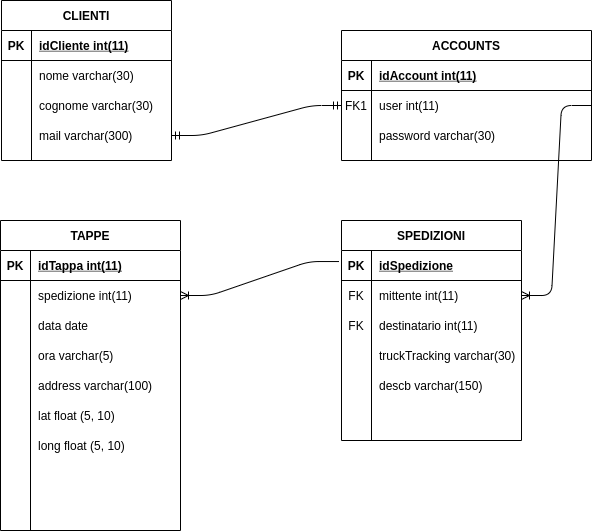
\includegraphics[scale=0.5]{img/er.png}
    \caption{Diagramma ER}
    \label{fig:my_label}
\end{figure}
Le entita’ strutturate nel DBMS sono 4.
\begin{enumerate}
    \item Per  ogni accounts vi e’ un solo cliente, un cliente puo’ avere un solo account;
    \item Per ogni accounts possono esserci svariate spedizioni, una spedizione puo’ appartenere al piu’ a un account;
    \item Per ogni spedizioni possono esistere molteplici tappe, una tappa appartiene solo e soltanto a una spedizione.
\end{enumerate}

\subsection{Panoramica sullo sviluppo infrastrutturale}
\begin{figure}[H]
    \centering
    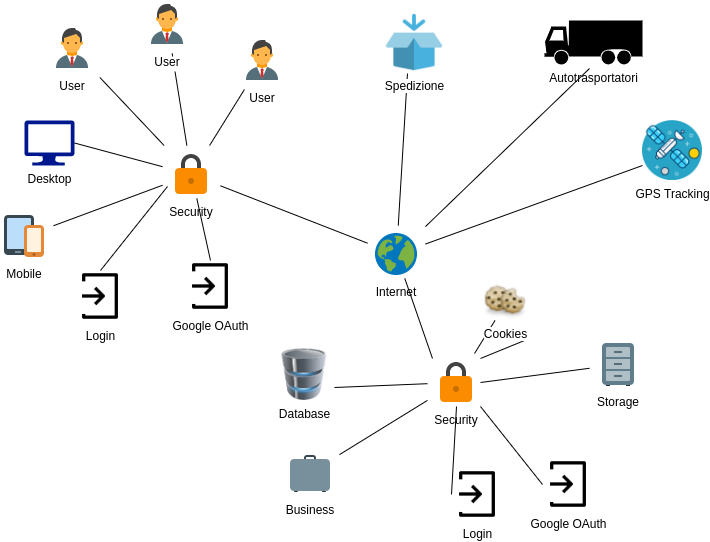
\includegraphics[scale=0.5]{img/pozzebonGrafic.png}
    \caption{Infrastruttura}
\end{figure}
\newpage

\subsection{Panoramica sulle librerie utilizzate} 

Per la realizzazione del sito e l’attivazione dei differenti servizi e’ stata necessaria l’implementazione di differenti librerie.\\
\href{https://getcomposer.org/}{Composer}, il Dependency Manager di Php e’ stato fondamentale in questa parte dello sviluppo.\\
\begin{enumerate}
    \label{label_api}
    \item Per la generazione delle coordinate dato l'indirizzo e' stato necessario attivare e implementare le \href{https://console.cloud.google.com/apis/library/geocoding-backend.googleapis.com}{Api Google per il Geocodig};
    \item Per la gestione del Google OAuth e’ stato necessario attivare e implementare le \href{https://developers.google.com/identity/protocols/oauth2}{Api Google per il Google Oauth};
    \item Per la generazione automatica dei Qr Code e’ stato necessario implementare la libreria \href{http://phpqrcode.sourceforge.net/}{PHP Qr Code};
    \item Per l’invio automatico della mail contenente il codice di conferma e’ stato necessario implementare \href{https://github.com/PHPMailer/PHPMailer}{PHPMailer}
\end{enumerate}
\subsection{Funzionalita' di sviluppo}
In fase di progettazione e’ stato deciso di suddividere quanto piu’ possibile le differenti funzionalita’. \\
La maggior parte delle funzioni e degli applicativi necessari e ricorrenti nel sito sono stati inseriti in un file header dedicato, chiamato \textit{func.php}.
\subsubsection{Connessione al database}
In quanto operazione piuttosto ricorrente e' stato deciso di creare una funzione ad hoc per la connessione al database.
\begin{lstlisting}[caption=\textit{connect()}]
<?php
    if(!isset($_SESSION))
        session_start();

$servername = "localhost";
$username = "root";
$password = "";
$db = "my_pozzebondelivery";

// Create connection
$conn = new mysqli($servername, $username, $password, $db);

// Check connection
if (@$conn->connect_error) {
    die("Connection failed: " . $conn->connect_error);
}																													
?> 
\end{lstlisting}

\subsubsection{Footer}
In ogni pagina e’ presente un footer indicante l’utente attivo in sessione un collegamento alla homepage del sito.

\begin{lstlisting}[caption=\textit{footer()}]
function footer(){

if(isset($_SESSION["user"])){
    $user = $_SESSION["user"]; 
}else $user = "";

echo "<div class=\"footerContainer\">
<br>
  <button class=\"homeBTN\" onclick=\"window.location.href=' "
  .url().
  " '\"> <b> Home [".$user."] </b> </button><br> <br>
  </div>";
}
            
\end{lstlisting}

\subsubsection{Aggiunta nuovo utente}
\begin{lstlisting}[caption=\textit{newUserInsert()}]
function newUserInsert($email, $pwd,  $nome, $cognome, $google){
include "connect.php";

$inserNewClienteQuery= "INSERT INTO clienti (nome, cognome, mail)
                 VALUES(\"$nome\",\"$cognome\",\"$email\")";
    
if (mysqli_query($conn, $inserNewClienteQuery)) {
    echo "";
}
else {
    echo "Errore Di Inserimento!".mysqli_error($conn);
}

    //getNewClientID
$loginQuery = "SELECT idCliente
FROM clienti
WHERE mail = \"$email\"";


$loginRes   = $conn->query($loginQuery);

$row   = $loginRes->fetch_assoc();
$_user  = $row["idCliente"];
echo $_user;

if(isset($_user)){ 
    $inserNewClienteQuery = "INSERT INTO account (user, password)
VALUES(\"$_user\", DES_ENCRYPT(\"$pwd\"))";

    if (mysqli_query($conn, $inserNewClienteQuery)) {
        login($email," ", $nome, $cognome, $google, 0);
    }
    else {
        echo "Errore Di Inserimento!".mysqli_error($conn);
    }
}       
}
                
\end{lstlisting}
\newpage
\subsubsection{Login}
Una procedura fondamentale e' quella del login.
\begin{lstlisting}[caption=\textit{login()}]
function login($user, $pwd, $nome, $cognome, $google){
    $_SESSION["user"]    = $user;
    $_SESSION["pwd"]     = $pwd;
    $_SESSION["nome"]    = $nome;
    $_SESSION["cognome"] = $cognome;
    $_SESSION["google"]  = $google;
    header("Location: areaPersonale.php");
}
\end{lstlisting}
\subsubsection{Logout}
\begin{lstlisting}[caption=\textit{login()}]
function logout(){
    if(isset($_SESSION["user"]) && isset($_SESSION["pwd"])){
        unset($_SESSION["user"]);
        unset($_SESSION["pwd"]);
        session_destroy();
        header("Location: login.php");
    }
    else { session_destroy(); header("Location: ../index.php");}
}
\end{lstlisting}
\subsubsection{Generazione Qr Code}
Per la generazione del Qr Code e' stato deciso di usare la libreria Phpqrcode per generare il file immagine nella cartella di riferimento \textit{img}.
\\Successivamente la funzione torna un vettore contenente due stringhe: il path completo fino all'imagine e l'url della pagina di visualizzazione della 
spedizione.
\begin{lstlisting}[caption=\textit{getQrCode()}]
function qrCode($id) {

    require_once "phpqrcode/qrlib.php";
    $path        = "../img/";
    $file        = $path.$id.".png";
    $url         = url()."src/sped.php?idSped=".$id;

    QRcode::png($url, $file, "L", 4, 4); 

return array($file, $url);
}
\end{lstlisting}
\subsubsection{Coordinate e Indirizzo geografico}
Grazie alle Api di Google Maps e' stato possibile calcolare in runtime il valore 
di latitudine e longitudine della tappa.\\ 
La funzione infatti, data la stringa d'indirizzo geografico, restituisce il valore \textit{float} delle coordinate attraverso un oggetto di classe \textit{Geocoding}.
\begin{lstlisting}[caption=\textit{getCoord()}]
function getCoord($addr){
    require "Geocoding.php";
    
    $geo = new Geocoding("<api key secret>");

    $cord = $geo -> getCoordinates($addr);

    return [ 'LT' => $cord['latitude'],
     'LO' =>  $cord['longitude']];
}
\end{lstlisting}
\subsubsection{Richiesta di trattamento cookie}
Il sito utilizza cookie di sessione. In linea con il nuovo GDPR e' stato quindi deciso di richiedere all'utente il permesso informato per la gestione 
delle proprie informazioni all'interno della sessione. \\
Questo compito e' stato affidato a una piccola funzione in JavaScript.\\
L'utente ha la possibilita' di scegliere, in caso contrario verra' reindirizzato a una simpatica gif e sara' impossibilitato ad utilizzare il sito.
\begin{lstlisting}[caption=\textit{cookies()}]
function cookies(){
<script type="text/javascript">	
    if(window.confirm("Questo sito usa i cookie vuoi continuare?") 
    && !Session["ookCok"]){
            Session["ookCok"] = true;
            window.location.href=".";
    }
    else{
        window.location.href=
        "https://i.giphy.com/media/BEob5qwFkSJ7G/giphy.webp";
    }
                
    </script>;
}
\end{lstlisting}
\subsection{Considerazione sulla sicurezza e la riservatezza dei dati}
All'interno del sito, come sovracitato, vi e' un utlizzo dei dati utente all'interno dei cookie di sessione; per ovviare a eventuali mancanze nel trattamento di questi dati l'utente e' prontamente informato.\\ 
Viene dunque richiesto il consenso \textit{esplicito} e \textit{informato} per tale utilizzo di informazioni; in caso contrario il sito non sara' accessibile. \\


All'interno del sito, piu' specificatemente nel database, vi e' anche l'archiviazione di password; e' stato quindi deciso di proteggere queste
informazioni salvando solamente l'hash della password attraverso una funzione \textit{sha256} e non la \\ chiave in chiaro. \\ 

Per garantire la cifratura della connessione e' stato deciso di usare un certifiato SSL per il portale. \\ 
Si tratta di un certificato generato con \href{https://www.openssl.org/}{OpenSSL}.

\subsection{Considerazioni e decisioni per l'hosting}
Data la natura del progetto e della complessita' di alcune funzionalita' le decisioni riguardo l'hosting sono cambiate diverse volte 
in fase di sviluppo. \\ La prima opzione, quella di utilizzare \href{https://it.altervista.org/}{Altervista},  e' stata scartata quasi subito. \\
Servizio ottimo per l'hosting di blog e affini ma scomodo se non addirittura controproducente per l'hosting di una piattaforma
come \textit{PozzebonSpedizioni}. La motivazione e' presto detta, su Altervista non e' possibile l'utilizzo di Composer, a noi indispensabile
per integrare ogni tipo di api e servizi esterni.

La scelta e' quindi ricaduta su \href{https://aws.amazon.com/free/?trk=ps_a134p000003yhhNAAQ&trkCampaign=acq_paid_search_brand&sc_channel=ps&sc_campaign=acquisition_IT&sc_publisher=google&sc_category=core&sc_country=IT&sc_geo=EMEA&sc_outcome=Acquisition&sc_detail=amazon%20aws&sc_content=Amazon%20AWS_e&sc_matchtype=e&sc_segment=455721528683&sc_medium=ACQ-P|PS-GO|Brand|Desktop|SU|AWS|Core|IT|EN|Text&s_kwcid=AL!4422!3!455721528683!e!!g!!amazon%20aws&ef_id=CjwKCAjwvMqDBhB8EiwA2iSmPChyXfcgliX39hxNQ-chnJF4pTgh37C5ky8iupvY3PSirs-CU-Xt7xoCjZgQAvD_BwE:G:s&s_kwcid=AL!4422!3!455721528683!e!!g!!amazon%20aws&all-free-tier.sort-by=item.additionalFields.SortRank&all-free-tier.sort-order=asc}{Amazon Aws}, 
la piattaforma proprietaria di Amazon che permette di affittare macchine virtuali con differenti prestazioni e sistemi operativi.

Nel nostro caso e' stato deciso di affidarsi a una EC2 - Debian Buster avente 8Gb di spazio sul disco, 2Gb di memoria Ram e 1 Core fisico. \\ 
Prestazioni piu' che sufficienti per il nostro utilizzo. \\ L'accesso alla macchina virtuale avviene grazie a una shell SSH autenticata tramite un file contenente una chiave secreta RSA generato al primo accesso.
E' proprio grazie alla potenza della shell a rendere questo servizio comodo e funzionale sotto ogni aspetto.

Il portale gestisce la fatturazione e i consumi della EC2 calcolando le ore di utilizzo e il numero di servizi abilitati, 
alla creazione dell'account offre 700 ore di utilizzo gratuito, completo di un indirizzo Ipv4 pubblico e servizio DNS.

\subsection{Portale Web e Demo}
Il sito e' quindi pubblico e accessibile qui:
\begin{itemize}
    \item \href{https://ec2-18-189-231-105.us-east-2.compute.amazonaws.com}{Pozzebon Delivery}
    \item \textit{ec2-18-189-231-105.us-east-2.compute.amazonaws.com}
\end{itemize}

Al fine di testare tutte le funzionalita' del sito sono stati  preventivamente creati due profili:
\begin{itemize}
    \item \textit{pozze.simo@gmai.com} - \textit{pozzesimo}
    \item \textit{rossi.mario@yahoo.it} - \textit{mariorossi}
\end{itemize}

\subsubsection{\textbf{Disclaimer}}
Il progetto e' vasto, e' quindi possibile trovare  bug e insuccessi durante la navigazione. \\
Alcune funzionalita’ di debug sono ancora attive per praticita'.\\ \\
L'azienda si scusa in anticipo! \\ Per ogni problema non esitare a contattare Simone:
\begin{itemize}
    \item \href{mailto:pozze.simo@gmai.com}{pozze.simo@gmail.com}
    \item \href{https://github.com/simopozze}{Git Hub}
\end{itemize}
\section{Conclusione}
Questo progetto mi ha segnato in positivo. \\ E' stato un brutto periodo e mi ero allontanato  dall'informatica,\\ \textit{Pozzebon Delivery} mi ha ridato 
la voglia di mettermi in gioco.

Le sfide sono state tante, cosi' come le soddisfazioni, per la prima volta mi e' capitato di utilizzare tecnologie
nuove (api, librerie PHP, ...) e spesso sono rimasto bloccato in un punto per giorni, mi sono anche aiutato parecchio grazie a forum e utenti 
conosciuti online.\\
Ne ho anche approfittato per studiare approfondire \LaTeX.
\end{document}
